\subsubsection{Human Tracking}
For human tracking and following, we implemented the TLD (Track-LearningDetection) algorithm [5]. TLD was proposed by Zdenek Kalal and is currently the state-of-art real time tracking algorithm. It combine the traditional tracking and detection algorithm so that it is more robust in consideration of distortion and partial occlusions. TLD algorithm consists of three modules as its name indicated. Tracking module estimate moving direction of the object according to the difference between two adjacent frames. Detection module detect the object in each frame independently. Learning module integrate the results of the tracking module and detection module to correct the detection errors and update the features of the target object.
We applied the TLD algorithm to human tracking and following tasks. Before the robot starts following, the human partner to be followed will be asked to stand in front of Kinect and the robot will record his/her features. When the instructor starts moving around, the robot will track and keep up with him. The robot also uses the depth information to keep away from the instructor at a safe distance.
\subsubsection{Face Recognition}
For human-robot interaction, a robot is required to recognize different masters or guests in home service. We developed a face recognition system with two process: enrollment and recognition. During the enrollment process, a man is asked to stand in front of the RGB camera. A face detector based on haar feature from OpenCV is applied and the detected face will be stored. For a single person, the system stores 3-5 pictures.
We implemented the face recognition algorithm based on sparse representation [4]. A redundant dictionary is trained offline using a set of training faces. The algorithm seeks the most sparse representation coefficient by solving a L1 optimization problem. The residual errors for different classes (persons) tell who is the unknown person: if the residual error for a specific class, for example, person A, is smaller than a specified threshold and the errors for other classes are larger than another specified threshold, the newcoming person is identified as person A. Fig.4 shows an example of the face recognition result.
\begin{figure}[H]
    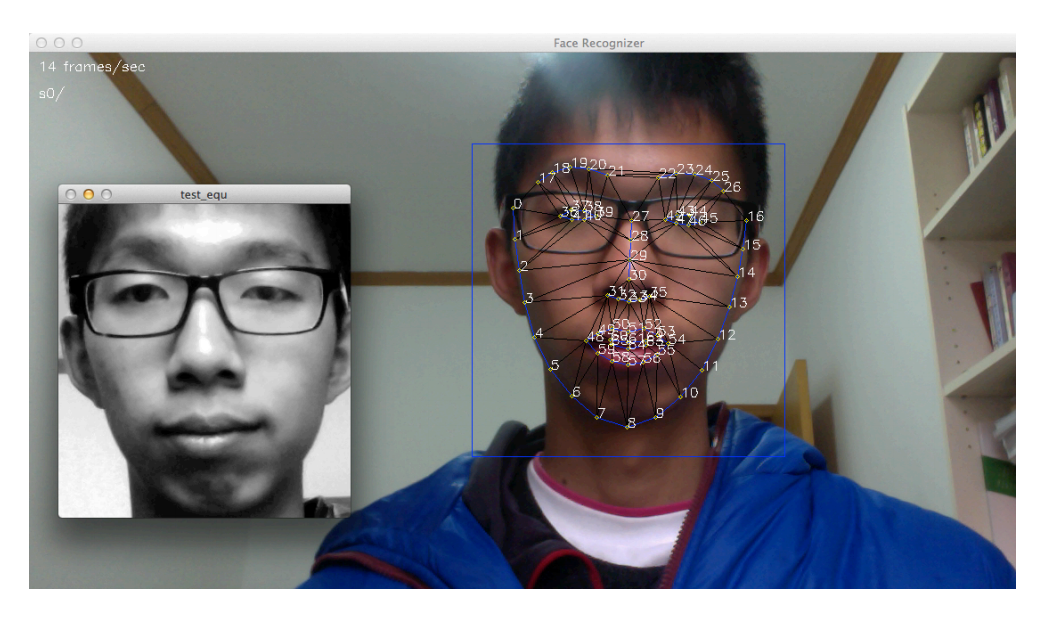
\includegraphics[scale=0.5]{face.png}
    \caption{face recognition}
\end{figure}
\subsubsection{Object recoginition and manipulation}
Tinker uses a two-phase approach to recognize objects and precisely manipulate them. In the first phase, a point cloud is built from the Kinect depth camera. Hough transform and an entropy-based filter is applied to the point cloud to remove the backgroud. Then a euclidean clustering will give the region of interest. A typical image of the filtered point cloud is given below:
\begin{figure}[H]
    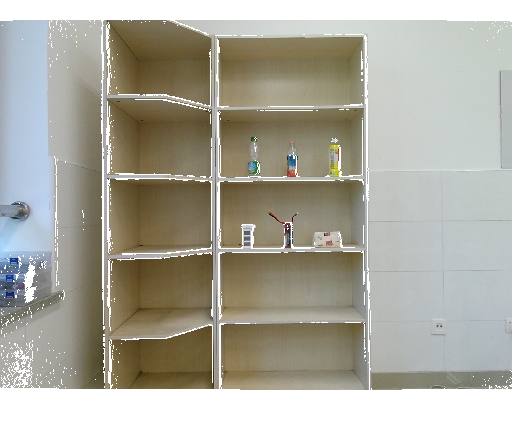
\includegraphics[scale=0.5]{original.png}
    \caption{original image}
\end{figure}

\begin{figure}[H]
    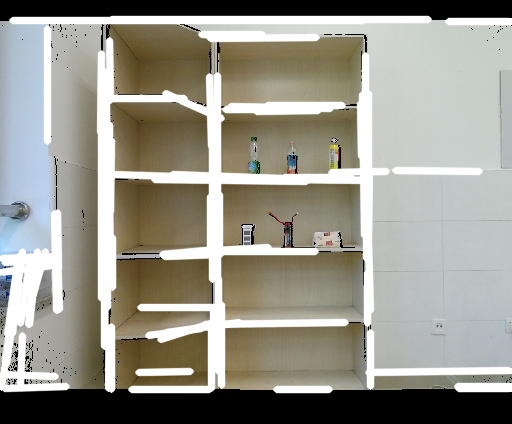
\includegraphics[scale=0.5]{filtered.png}
    \caption{filtered image}
\end{figure}

In the second phase, the approximate location of object is given to the robot arm controller, another usb camera placed in the hand of the robot arm will guide the arm to precisely manipulate the object. First, the hand is moved to directly face the location of the region of interest at about 40 cm away. A similar image processing pipeline is used to find the object in the image given by the camera in hand. After getting the image of the object, it is matched with the pre-captured image set by convolution the image with the templates to find the best mattch. Precision of the location found in this phase is significantly improved due to a much closer camera place. Then the robot arm will be guided by the camera using a feedback procedure to place the object in the middle of the camera image. Thus, the chance of missing the object is reduced.

\begin{figure}[H]
    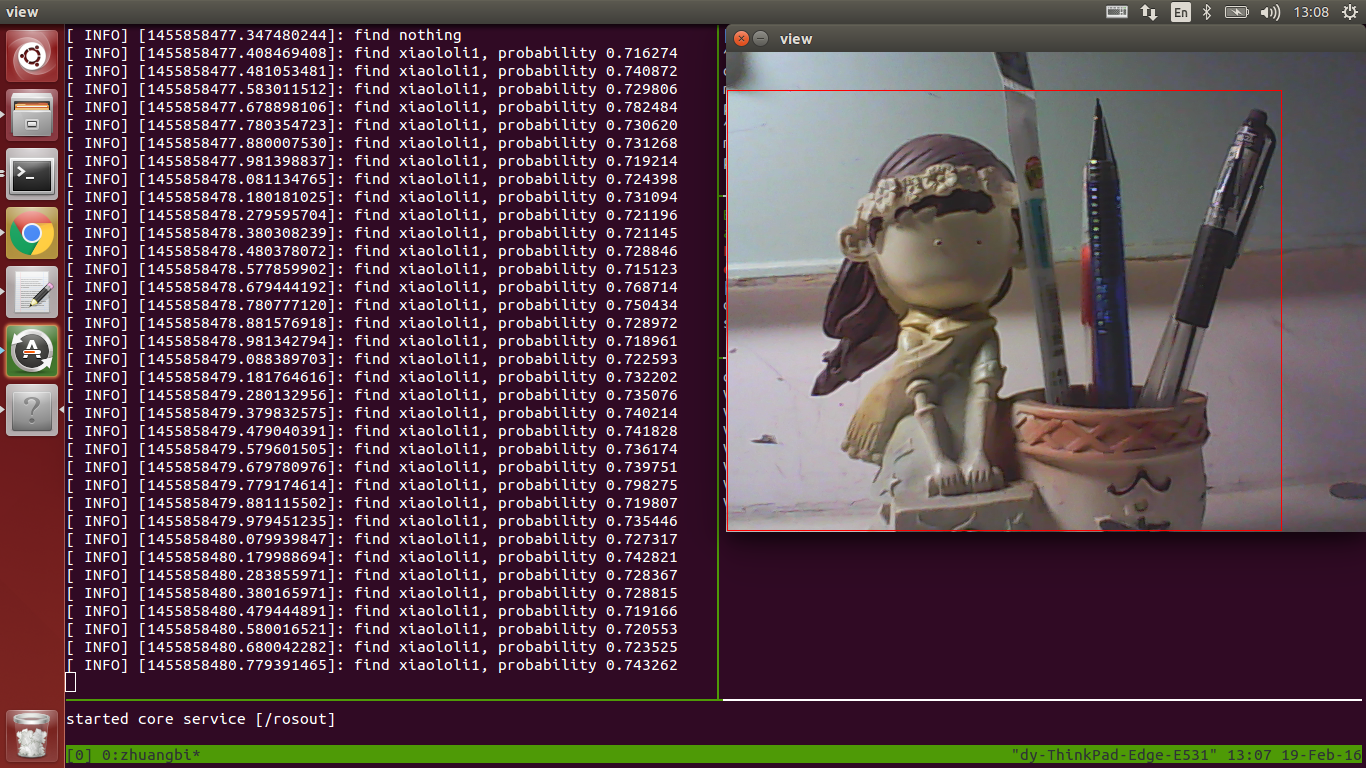
\includegraphics{object_found.jpg}
    \caption{object found from the camera}
\end{figure}
